\chapter{Introduction}
% The goal of this chapter is to give an overview of the available knowledge about stearoyl-CoA desaturase (SCD1) which is the main focus of this thesis. SCD1 is an iron-containing enzyme and member of the large non-heme iron enzyme family. The chapter starts  explaining the role of iron in biological systems and moves on to discuss the experimental and theoretical methods used to study non-heme iron enzymes. An overview of the rich chemistry of both binuclear and mononuclear non-heme iron enzymes is given before discussing the reactivity and importance of SCD1.

\section{Role of phosphates in biological systems}
Phosphates are among the fundamental building blocks that play a central role in life on Earth. They form the basis for both the storage and transfer of genetic information, as well as the flow of metabolic energy within biological systems. The ubiquitous nature of phosphate esters and anhydrides—such as those found in deoxyribonucleic acid (DNA), ribonucleic acid (RNA), adenosine triphosphate (ATP), and polyphosphate (polyP)—highlights their fundamental importance \citep{westheimerWhyNatureChose1987}. Some of the phosphates found in biological systems and their respective functions are summarised in Table~\ref{tab:role_of_phosphates}.

A key characteristic enabling these roles is the ability of phosphoric acid to link molecular units while retaining an ionisable group. This inherent negative charge at physiological pH serves a dual purpose: it helps to retain these molecules within cellular boundaries defined by lipid membranes, and more importantly, it confers kinetic stability upon phosphate esters and anhydrides by electrostatically repelling nucleophilic attack, particularly from water \citep{westheimerWhyNatureChose1987}. For instance, the half-time for hydrolysis at 25\textdegree{C} for a phosphomonoester monoanion (P–O) is about 90 years; however, for a phosphodiester anion (P–O), this number increases dramatically to approximately 16 million years \citep{wolfendenDegreesDifficultyWaterConsuming2006}. This stability is crucial for maintaining the integrity of genetic material but can be readily overcome by enzymatic catalysis when there is a metabolic demand.

Phosphates are involved in numerous processes in living systems, such as cell signalling and sensation, regulation of metabolism, blood coagulation, and bone formation \citep{mullerInorganicPolyphosphatesStorage2019, nebesnayaInorganicPolyphosphateRegulates2024}. Their role is perhaps most evident in cellular energetics, where ATP functions as the universal energy currency. The energy derived from nutrients such as glucose is captured and stored within the high-energy phosphoanhydride bonds linking the phosphate groups of ATP. This energy is released upon hydrolysis of the terminal phosphoanhydride bond (P-O bond between $\beta$ and $\gamma$ in Figure~\ref{fig:atp}), typically yielding adenosine diphosphate (ADP) and inorganic phosphate (P\textsubscript{i}). The cleavage of this bond provides the thermodynamic driving force for the majority of cellular processes, including biosynthesis, active transport, and mechanical work such as muscle contraction. The standard free energy change for ATP hydrolysis is substantial ($\Delta G^{0}=-30.5$ kJ mol$^{-1}$), and under cellular conditions, the actual free energy release is often considerably greater. Specifically, the experimentally obtained $\Delta G$ values are approximately $-59$ to $-53.5$ kJ mol$^{-1}$ in the liver and about $-61.7$ to $-59.5$ kJ mol$^{-1}$ in the heart \citep{mullerInorganicPolyphosphatesStorage2019}.

\begin{table}[b!]
    \centering
    \begin{tabular}{cc}
    \toprule
    \textbf{Phosphate} & \textbf{Biological role} \\ 
    \midrule
    DNA/RNA & Genetic material \\
    ADP/ATP & Intracellular energy transfer \\
    cAMP & Cellular signalling \\
    Polyphosphate & Energy storage, Cellular signalling \\
    Creatine phosphate & Intracellular energy transfer \\
    Phosphoenolpyruvate & Metabolism \\
    Pyridoxal phosphate & Coenzyme \\
    Nicotine adenine dinucleotide & Calcium signalling \\
    Fructose 1,6-diphosphate & Metabolism \\
    Glucose-6-phosphate & Metabolism \\
    Isopentenyl pyrophosphate & Metabolism \\
    Ribose-6-phosphate & Metabolism \\
    Glycerol 3-phosphate & Metabolism \\
    Dihydroxyacetone phosphate & Calvin cycle, metabolism \\
    Inositol phosphates & Cellular signalling \\
    \bottomrule
    \end{tabular}
    \caption{Examples of biologically relevant phosphates and their roles. Reproduced and adapted from~\citep{kamerlinWhyNatureReally2013}.}
    \label{tab:role_of_phosphates}
\end{table}

Beyond ATP, inorganic polyphosphate (polyP)—a linear polymer of orthophosphate residues linked by similar high-energy phosphoanhydride bonds—represents another significant phosphate-based energy storage found across all domains of life, including mammalian cells. However, in mammalian cells, the concentration of polyP is significantly lower compared to that in microorganisms. While its roles in mammals are still being fully elucidated, polyP metabolism is intrinsically linked to the cellular energy status. Mitochondrial polyP levels fluctuate with respiratory activity and appear to depend on F\textsubscript{0}F\textsubscript{1}-ATP synthase function, suggesting a role in mitochondrial bioenergetics, potentially acting as an energy reservoir \citep{pavlovInorganicPolyphosphateEnergy2010}.

The efficient transfer of energy stored in phosphate bonds from sites of production (e.g., mitochondria) to sites of utilisation (e.g., ATPases involved in muscle contraction or ion transport) is crucial. Simple diffusion of ATP is often insufficient due to the complexity of intracellular architecture and the potential for large concentration gradients to arise, which would be thermodynamically inefficient. Instead, cells employ phosphotransfer networks, utilising enzymes such as creatine kinase and adenylate kinase, which catalyse phosphoryl exchange reactions. These networks act as 'phosphoryl wires', facilitating the efficient conduction of high-energy phosphoryl groups and energetic signals throughout the cell with minimal energy dissipation or accumulation of inhibitory products such as ADP. The existence of these networks underscores the dynamic and highly organised nature of cellular energy management, where phosphates—mainly in the form of ATP—serve as the key energy carriers \citep{dzejaPhosphotransferNetworksCellular2003}.

The synthesis of ATP occurs primarily through oxidative phosphorylation in mitochondria, a process tightly coupled to the electron transport chain, which establishes a proton-motive force ($\Delta p$) across the inner mitochondrial membrane. This electrochemical potential energy is used by the molecular machine ATP synthase. Interestingly, the principal energy input required by ATP synthase is not for the chemical formation of the phosphoanhydride bond itself, but rather for the conformational changes necessary to release the newly synthesised, tightly bound ATP molecule from the enzyme's catalytic site. This 'binding change mechanism' involves the cooperative, sequential action of the enzyme's multiple catalytic sites, driven by proton flow. The hydrolysis of ATP to ADP and P\textsubscript{i} is catalysed by a variety of enzymes, including ATPases and possibly F\textsubscript{1}-ATPase, which are frequently coupled to other cellular processes \citep{boyerEnergyLifeATP1998}.

In essence, the unique chemical properties of phosphates—their ability to form stable esters and energy-rich anhydrides, along with their negative charge—combined with the evolution of sophisticated enzymatic machinery for their synthesis, transfer, and hydrolysis, have secured their vital role in virtually all life processes.



\section{Enzymes involved in phosphate hydrolysis}
The hydrolysis of high-energy phosphoanhydride bonds, particularly the terminal bond in adenosine triphosphate (ATP), is a cornerstone of cellular bioenergetics. While numerous enzymes utilise ATP hydrolysis, the F\textsubscript{0}F\textsubscript{1}-ATP synthase complex, primarily known for synthesising ATP, also shows potential ATP hydrolytic activity, particularly through its F\textsubscript{1} component (F\textsubscript{1}-ATPase). This enzyme complex, therefore, plays a dual role in managing the cell's primary energy currency \citep{bonoraATPSynthesisStorage2012, boyerEnergyLifeATP1998, walkerATPSynthaseUnderstood2013}. Furthermore, recent evidence suggests that this complex may also participate in the metabolism, including the hydrolysis, of inorganic polyphosphate (polyP) in mammalian cells \citep{baevInorganicPolyphosphateF0F1ATP2022, baevInorganicPolyphosphateProduced2020}.

The F\textsubscript{0}F\textsubscript{1}-ATP synthase is a molecular motor embedded in the mitochondrial membrane. It consists of two major domains: the F\textsubscript{1} domain, which carries the catalytic sites, and the F\textsubscript{0} domain, which is embedded within the membrane. These domains are connected by a central rotor stalk and a peripheral stator stalk \citep{walkerATPSynthesisRotary1998, walkerATPSynthaseUnderstood2013, wattBioenergeticCostMaking2010}. The activity of this enzyme is coupled with the electron-transport chain, as illustrated in Figure~\ref{fig:atp_synthase}.

\begin{figure}[t!]
    \centering
    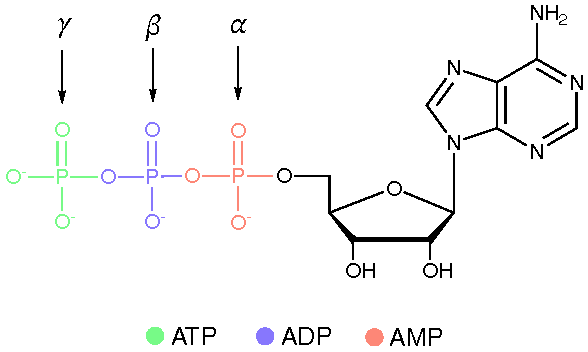
\includegraphics[width=0.6\textwidth]{Figures/1_Introduction/intro_atp.pdf}
    \caption{Chemical structures of the AMP, ADP, and ATP molecules with the phosphates marked as $\alpha$, $\beta$, and $\gamma$, respectively.}
    \label{fig:atp}
\end{figure}

The F\textsubscript{1} domain ($\alpha_3\beta_3\gamma\delta\epsilon$ stoichiometry) extends into the mitochondrial matrix. It has a globular shape as can be seen in Figure~\ref{fig:atp_synthase}. The catalytic sites for ATP synthesis and hydrolysis are located on the three $\beta$ subunits, which interact with the $\alpha$ subunits. When functioning in reverse, the F\textsubscript{1} domain acts as an F\textsubscript{1}-ATPase, hydrolysing ATP. This hydrolysis drives the counterclockwise rotation (as viewed from the membrane) of the central stalk, composed of the $\gamma$, $\delta$, and $\epsilon$ subunits \citep{walkerATPSynthesisRotary1998, walkerATPSynthaseUnderstood2013, boyerEnergyLifeATP1998}. If coupled to the F\textsubscript{0} domain, this rotation actively pumps protons from the matrix, thereby generating or maintaining the proton-motive force ($\Delta p$). This reverse function is especially important under conditions of low $\Delta p$, where it helps prevent its complete dissipation at the expense of cellular ATP and possibly polyP \citep{bonoraATPSynthesisStorage2012, walkerATPSynthaseUnderstood2013, baevInorganicPolyphosphateProduced2020}.

The mechanism of ATP hydrolysis (cleavage of the P–O bond between $\beta$ and $\gamma$ in Figure~\ref{fig:atp}) follows the principles of the binding change mechanism \citep{walkerATPSynthaseUnderstood2013}. The rotation of the asymmetric $\gamma$ subunit induces sequential conformational changes in the three $\beta$ subunits, cycling them through states analogous to those in synthesis: an 'open' state that binds ATP, a 'tight' state that facilitates hydrolysis, and a subsequent 'open' state that releases ADP and P\textsubscript{i} \citep{walkerATPSynthesisRotary1998, boyerEnergyLifeATP1998}. The hydrolysis of each ATP molecule is associated with a 120\textdegree{} rotation of the central stalk, which occurs in substeps \citep{walkerATPSynthaseUnderstood2013}.

While the metabolism of inorganic polyphosphate (polyP) is well-characterised in microorganisms via specific kinases (PPK) and phosphatases (PPX), the enzymes responsible for its turnover in mammalian cells remain largely unknown. Recent studies using immunocaptured F\textsubscript{0}F\textsubscript{1}-ATPase have demonstrated that the enzyme complex can hydrolyse polyP. This polyP hydrolysis appears to drive the enzyme's proton-pumping activity, akin to ATP hydrolysis, and is sensitive to oligomycin, a specific F\textsubscript{0}F\textsubscript{1}-ATP synthase inhibitor. Medium- and long-chain polyP molecules, made of 60 and 130 orthophosphate units, respectively, seem to be effective substrates for this hydrolytic activity. Docking simulations support the feasibility of polyP binding to the nucleotide-binding sites within the F\textsubscript{1} domain. This suggests that polyP could serve as an alternative energy source for the F\textsubscript{0}F\textsubscript{1} complex, potentially helping to maintain mitochondrial membrane potential when ATP levels are compromised \citep{baevInorganicPolyphosphateProduced2020, baevInorganicPolyphosphateF0F1ATP2022}.

\begin{figure}[t!]
    \centering
    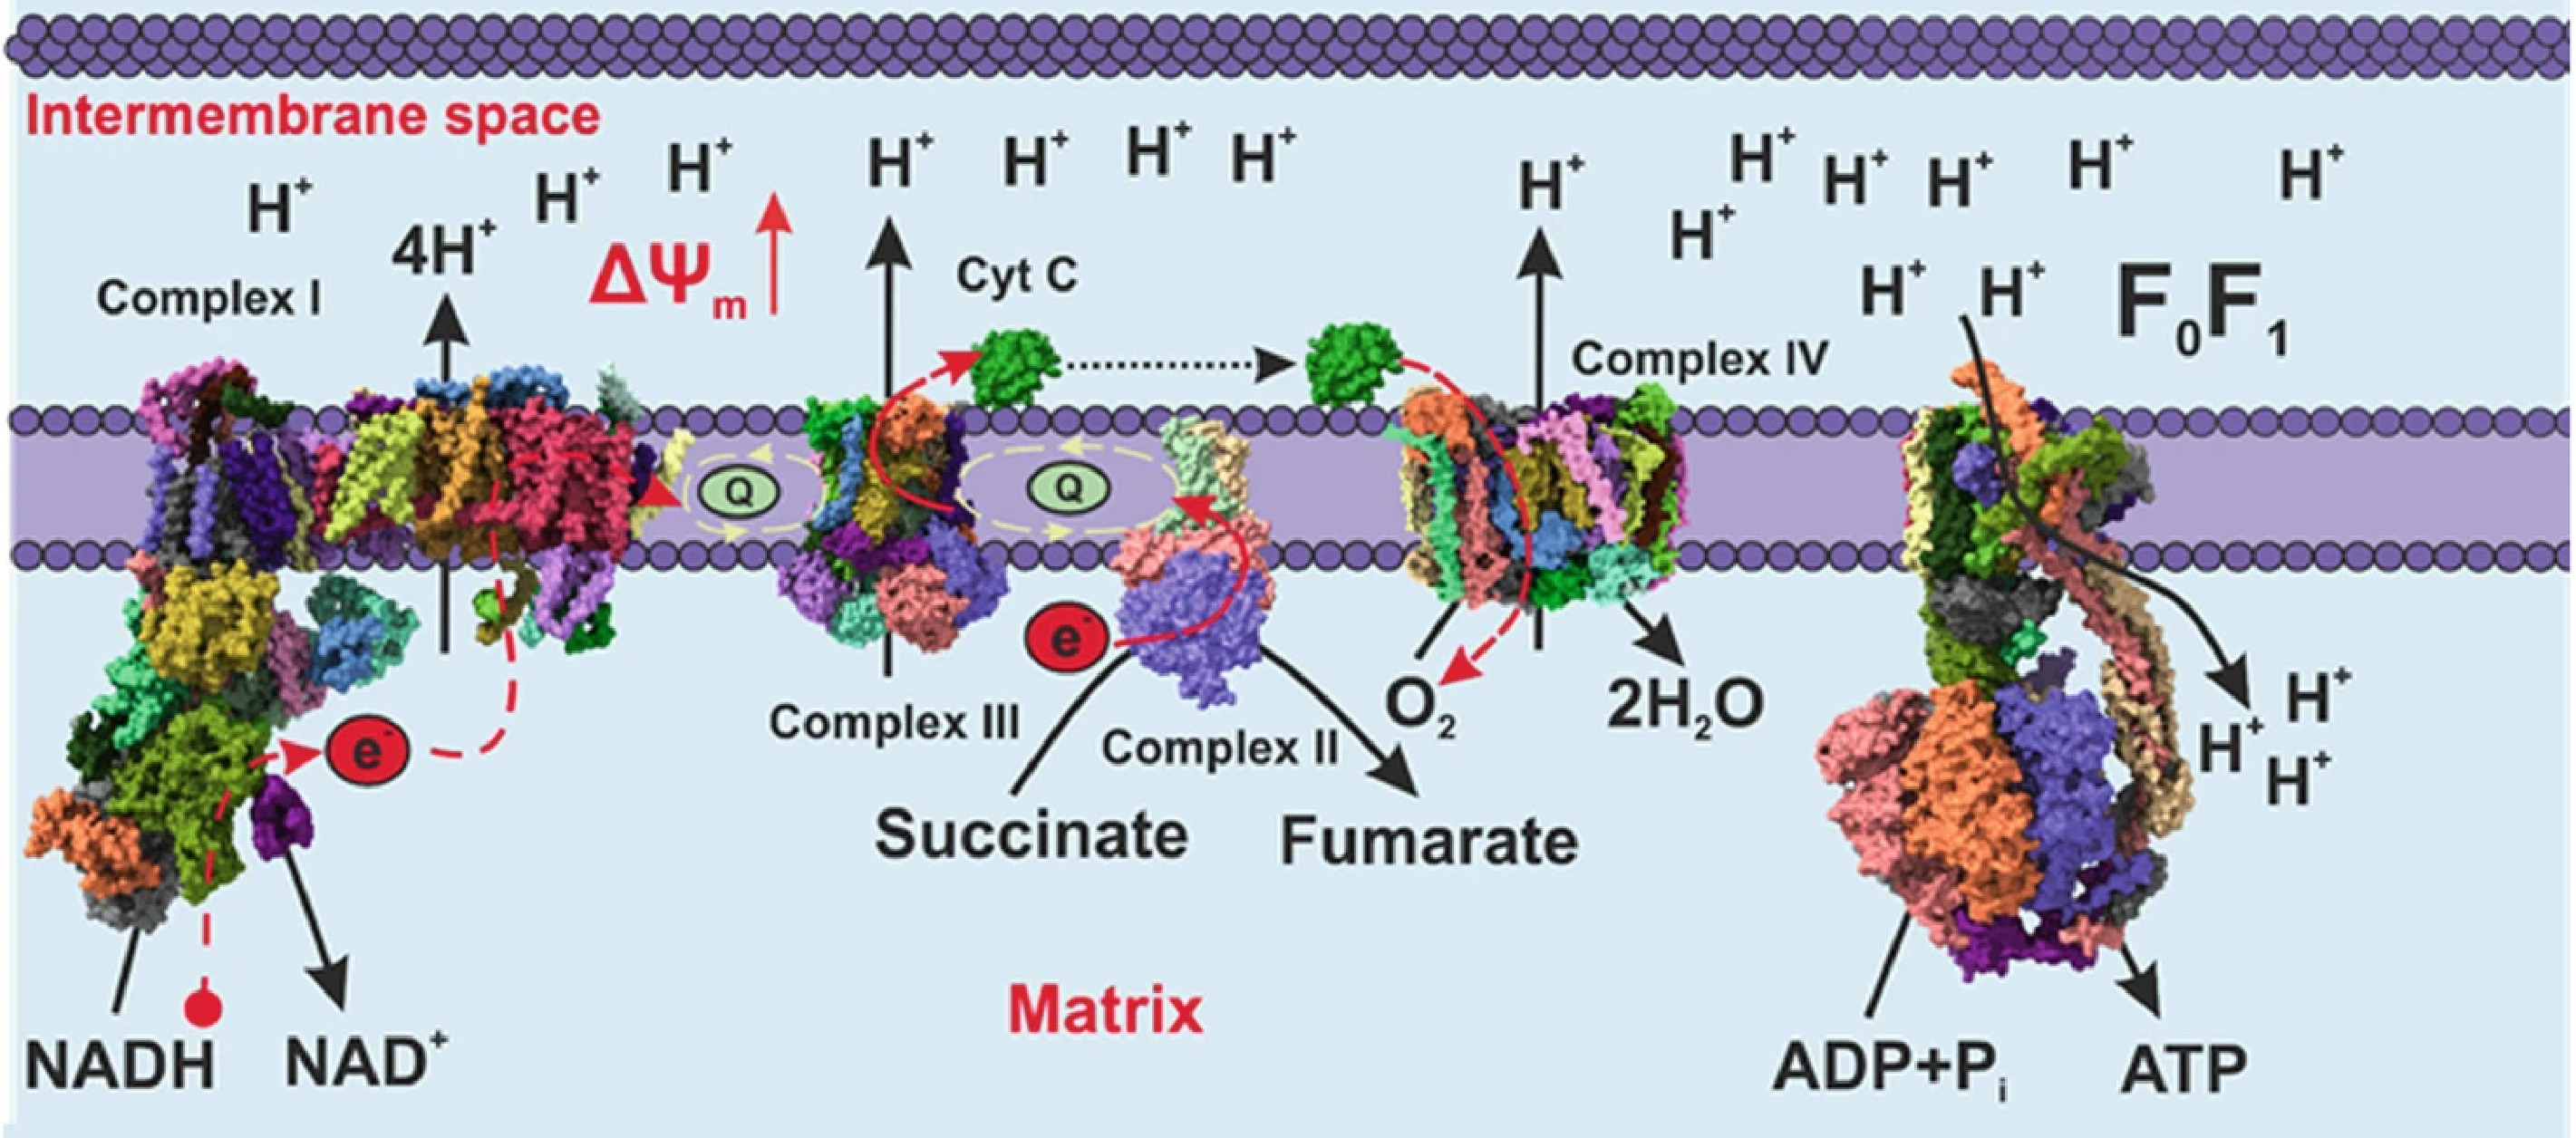
\includegraphics[width=0.95\textwidth]{Figures/1_Introduction/intro_atp_synthase.pdf}
    \caption{Electron transport chain coupled with oxidative phosphorylation in mitochondria. Reproduced from \citep{baevInorganicPolyphosphateF0F1ATP2022}.}
    \label{fig:atp_synthase}
\end{figure}

There is growing confidence that the F\textsubscript{1}-ATPase could act not only as an ATP hydrolase but also potentially as a polyP hydrolase. However, other enzymes contribute to phosphate metabolism as well. In the context of polyP, mammalian enzymes such as alkaline phosphatase (ALP) have demonstrated exopolyphosphatase activity, capable of degrading polyP chains of various lengths \citep{baevInorganicPolyphosphateF0F1ATP2022}.

The world of enzymes—and phosphate hydrolysis by F\textsubscript{1}-ATPase in particular—is both fascinating and complex. The F\textsubscript{1}-ATPase is a molecular machine capable of hydrolysing ATP and polyP, yet the precise mechanism of hydrolysis remains not well understood. In order to address this gap, it is necessary to investigate the fundamental reaction mechanisms of phosphate hydrolysis, beginning with the simplest phosphate esters in less complex environments such as bulk water.



\section{Reaction mechanism}

\begin{figure}[htbp]
    \centering
    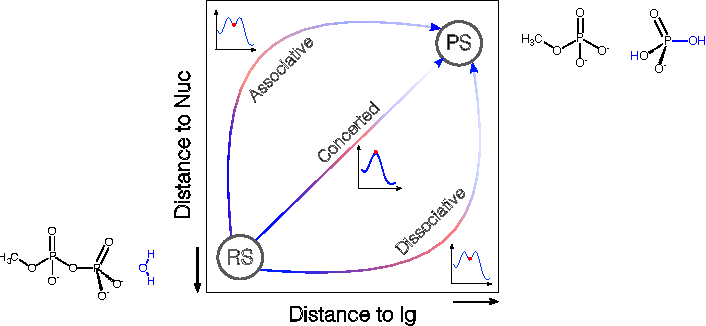
\includegraphics[width=0.5\textwidth]{Figures/1_Introduction/intro_mfj_plot.pdf}
    \caption{MFJ plot.}
    \label{fig:mfj_plot}
\end{figure}

\subsection{S\textsubscript{N}1 and S\textsubscript{N}2 nucleophilic substitution reactions}

\begin{figure}[htbp]
    \centering
    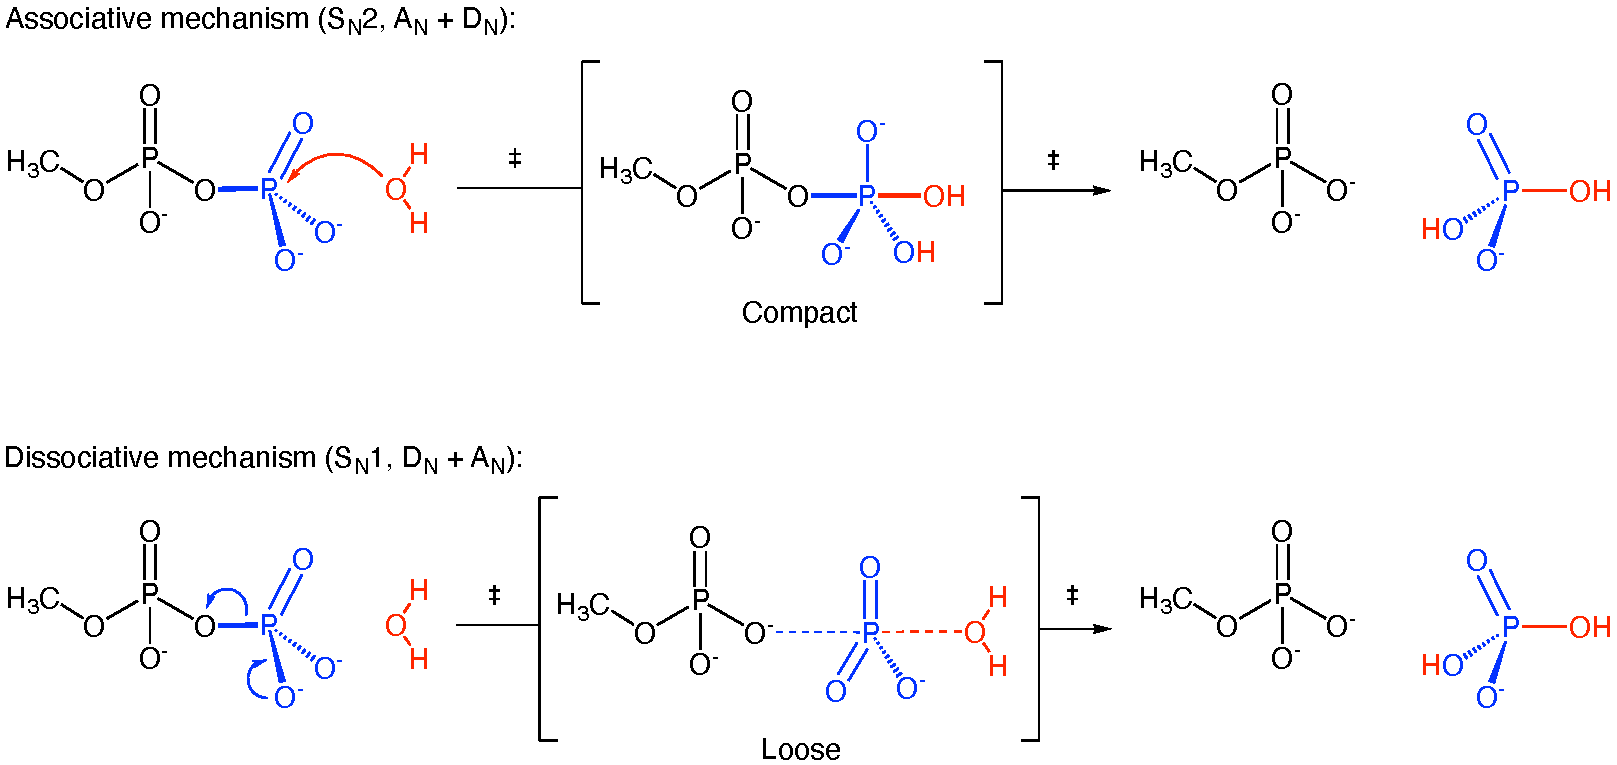
\includegraphics[width=0.95\textwidth]{Figures/1_Introduction/intro_reaction_mechanism.pdf}
    \caption{Reaction mechanism.}
    \label{fig:reaction-mechanism}
\end{figure}


\section{Research goals}


